\subsection{Results}
This section is still subject to change as findings reveal advantages and drawbacks
of parameter choices.
Three choices of clustering algorithm are considered here;
\begin{itemize}
    \item A standard anti-KT algorithm with \(\stoppingdeltar{}=1.36\)
    \item A \spectralfulljet{} algorithm with \(2\) eigenvectors, \(\stoppingdeltar{}=0.63\), and \(q=-0.035\)
    \item A \spectralmeanjet{} algorithm with \(4\) eigenvectors, \(\stoppingdeltar{}=0.70\), and \(q=0\)
\end{itemize}

As the data is simulated it is possible to compare the performance of clustering algorithms to Monte Carlo truth.
Each event contains 4 \bthing{quarks} and for each of them it is possible to identify the particle into which they decayed, as a subset of the particles in the final state.
Henceforth the detectable decay products of the \bthing{quark} will be called the descendants of the \bthing{quark}.
For two reasons it is not possible for this clustering algorithm to gather all the descendants
of each \bthing{quark} into one jet:
firstly not all the descendants make the \(p_T\) and \(\eta\) cuts, so some are discarded  before clustering;
secondly the descendants of the \bthing{quarks} in an event are not mutually exclusive, due to interactions during hadronisation the quarks share descendants, and our clustering algorithm does produce exclusive clusters.

Knowing the parts of the final state that are descended from each \bthing{quark} creates a clear
allocation of jets to quarks.
For each quark, the jet that contains the greatest mass in descendent particles is tagged to represent that quark.

Mass peaks can the be constructed from the tagged jets, using all the particles in the jet,
both descendant of the quarks and background.
In figure~\ref{fig:best_all} the masses of all jets that have been \bthing{tagged} are plotted.
In figure~\ref{fig:best_correct_h_allocation} three selections are plotted; firstly only events where some trace of all 4 \bthing{quarks} is found
are plotted with the mass of the descendants of the heavy Higgs in the background.
Then the two light Higgs in each event are sorted by the mass of their descendants,
in effect they are ranked by how well they were picked up by the detector.
The mass of the light descendants is plotting in the background and over
that the mass of the associated jets in each event is shown.


\begin{figure}[htp]
    \begin{minipage}[c]{0.5\textwidth}
        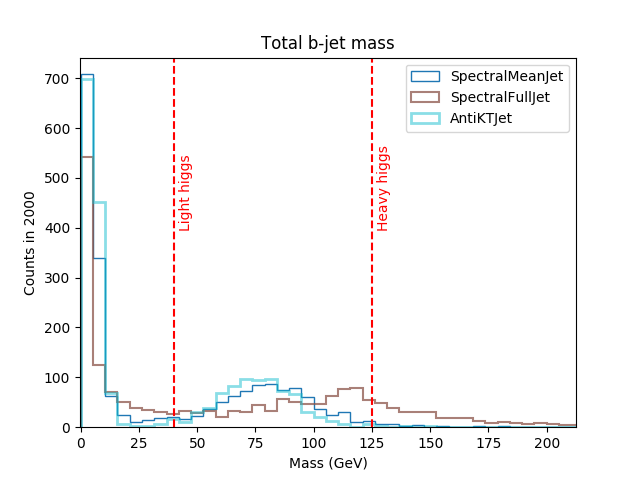
\includegraphics[width=1\textwidth]{graphics/best_all.png}
    \end{minipage}\hfill
    \begin{minipage}[c]{0.45\textwidth}
        \caption{All tagged jets in each event are plotted.
            A peak just shy of \(125\)GeV is desired as this is the mass of the decaying
            heavy Higgs.
            Another peak at \(40\)GeV could be observed is only one light Higgs
            was found in the detector volume.
            \spectralfulljet{} gets closest, peaking close to \(115\) GeV and
            showing some contamination from background with the bins \(>125\) GeV.
            Anti-KT and \spectralmeanjet{} both give similar behaviour, falling somewhat short.
            The Anti-kt jet used a \stoppingdeltar{} of \(0.63\).
        }\label{fig:best_all}
    \end{minipage}
\end{figure}    


\begin{figure}[htp]
    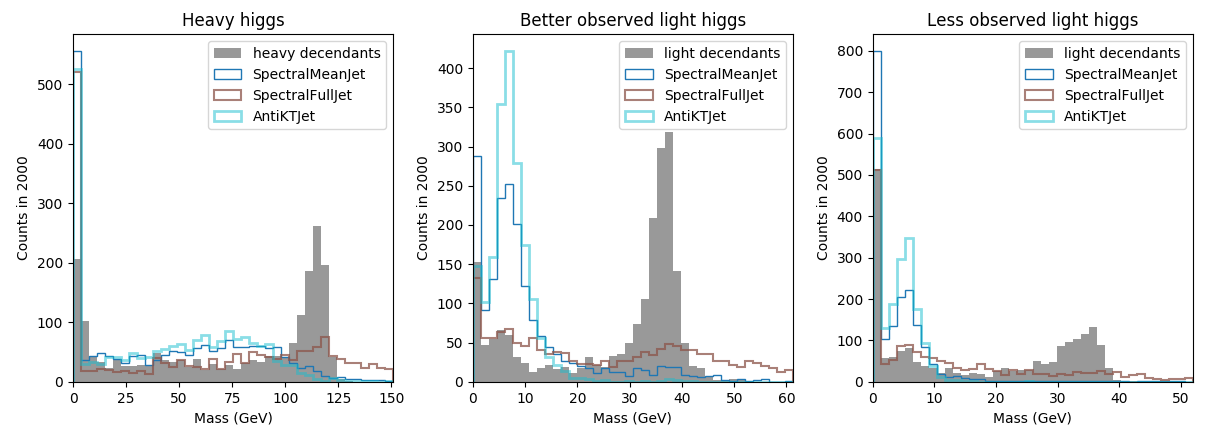
\includegraphics[width=1.\textwidth]{graphics/best_correct_h_allocation.png}
    \caption{Starting with the plot on the far left, the jet mass of events where
        some descendants from all 4 \bthing{quarks} were found is plotted over
        the total mass of all descendants.
        The plot in the centre takes the light Higgs whose descendants have the greatest mass in each event.
        The mass of these descendants is plotted in grey, and over this
        the masses of the jets in each event that correspond to this better observed Higgs
        are shown.
        That is, the tags in each event that have been produced by the better observed light Higgs
        are allocated to jets, and only the mass of these jets is tabulated - thus
        a good cluster will have obtained the mass of the light Higgs descendants.
        Finally on the left the light Higgs who's descendants have less mass is shown along with
        the corresponding jets.
        These three plots make it clear that only \spectralfulljet{} is obtaining the majority of the
        descendants, but it is combining them with some background as the tail of the
       \spectralfulljet{} distribution continues past the descendants distribution
       out of the frame.
       The behaviour of \spectralmeanjet{} does not significantly differ from Anti-KT
    }\label{fig:best_correct_h_allocation}
\end{figure}    
